
\documentclass{beamer}
%
% Choose how your presentation looks.
%
% For more themes, color themes and font themes, see:
% http://deic.uab.es/~iblanes/beamer_gallery/index_by_theme.html
%
\mode<presentation>
{
  \usetheme{default}      % or try Darmstadt, Madrid, Warsaw, ...
  \usecolortheme{whale} % or try albatross, beaver, crane, ...
  \usefonttheme{default}  % or try serif, structurebold, ...
  \setbeamertemplate{navigation symbols}{}
  \setbeamertemplate{caption}[numbered]
  \setbeamercolor{structure}{fg=beamer@miptblue}
} 

\usepackage[english]{babel}
\usepackage[utf8x]{inputenc}
\usepackage{xcolor}
\usepackage{ wasysym }

\definecolor{perovcolor}{HTML}{FED68F}
\definecolor{silicolor}{HTML}{D3D98C}
\definecolor{whalecolor}{HTML}{4C79BC}
\definecolor{beamer@miptblue}{HTML}{0072bc}
\definecolor{beamer@fopfblue}{HTML}{4c71b7}
\title[Blah blah]{robotics }
\author{}
\institute{MIPT, 325}
\date{}
\begin{document}

%\begin{frame}
%  \titlepage
%\end{frame}

\begin{frame}
\centering
\textcolor{beamer@fopfblue}{\Huge \quad \quad \quad Evgenii} \textcolor{beamer@miptblue}{\Huge Safronov \quad \quad~~}  
\newline
\newline{}
\includegraphics[width=0.23\textwidth]{Pictures/2_FOPF_color} \quad

\includegraphics[width=0.3\textwidth]{Pictures/eng}
\end{frame}
\section{MIPT}
\begin{frame}{\quad \quad ~Moscow Institute of Physics and Technology}
\textit{Well-known as Phystech}  \newline
School years: \underline{Physics}, \underline{Astronomy}, Programming, Math
\begin{columns}

\begin{column}{.59 \textwidth}
\begin{itemize}
  \item $\Rightarrow$ entered DGAP in 2013 
  \item \textbf{"Abramovka" scholarship} for excellent study
  \item \textbf{NIX scholarship} for best results on programming courses
  \item Diploma with honors, \textbf{4.92} GPA
  \item graduated in 2017
\end{itemize}
\centering
\vspace{0.1cm}
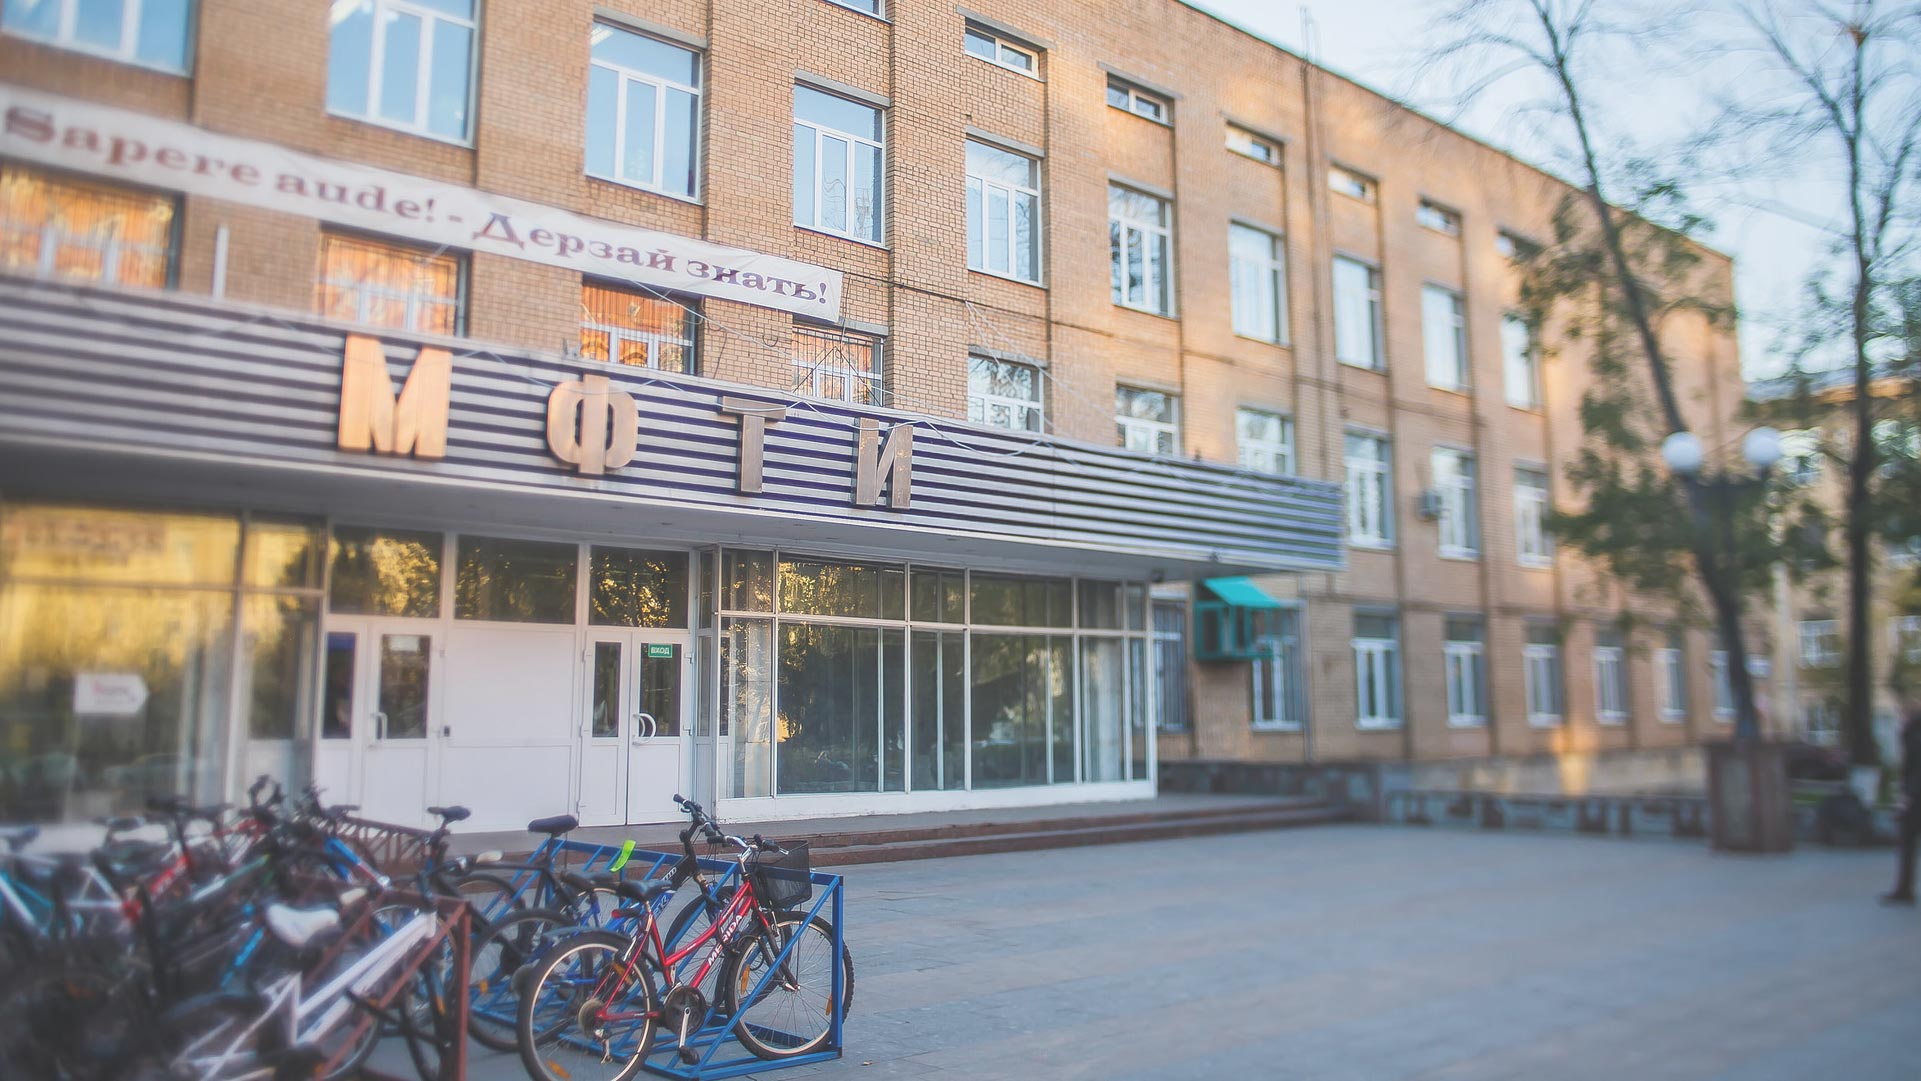
\includegraphics[width=0.8\textwidth]{Pictures/MIPT}
\end{column}
\begin{column}{.39 \textwidth}
Programming: \newline{} \newline{}
\quad \underline{3 compulsory} + \newline{}
\quad \underline{2 elective} programming courses + \newline{}
\quad \underline{6 extra} programming courseworks = \newline{}
\quad always \textbf{excellent} marks \newline{}

\end{column}
\end{columns}
\end{frame}


\section{Diploma}
\begin{frame}{\quad \quad ~Thesis}
\centering
``Single and Double Qubit Gates Optimization''
\vskip 0.1cm
\begin{columns}
\begin{column}{0.49\textwidth}
\centering
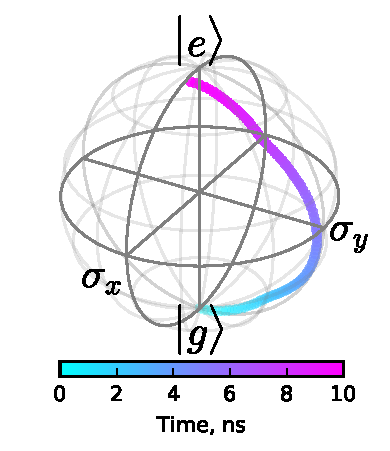
\includegraphics[width = 0.9\textwidth]{Pictures/bloch_incorrect_sy.pdf}
\end{column}
\begin{column}{0.49\textwidth}
\centering
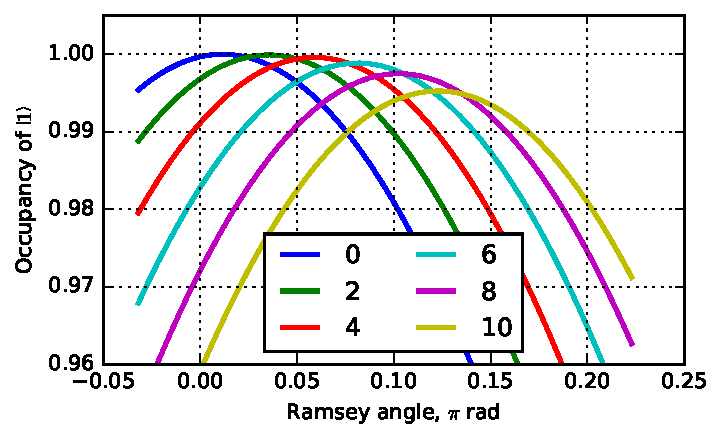
\includegraphics[width = 0.9\textwidth]{Pictures/APE_result_2.pdf}
\end{column}
\end{columns}
\vskip 0.1cm
\underline{https://github.com/safoex/qubitlab/}
\end{frame}


\section{Summer School Programme}
\begin{frame}{\quad \quad ~Summer School Programme}
\begin{columns}
\begin{column}{0.39\textwidth}
\centering

\includegraphics[width = 0.9\textwidth]{Pictures/hzb_logo_cmyk} \newline
2 months \newline 
\vskip 0.05cm
Poster presentation \newline
\vskip 0.1cm
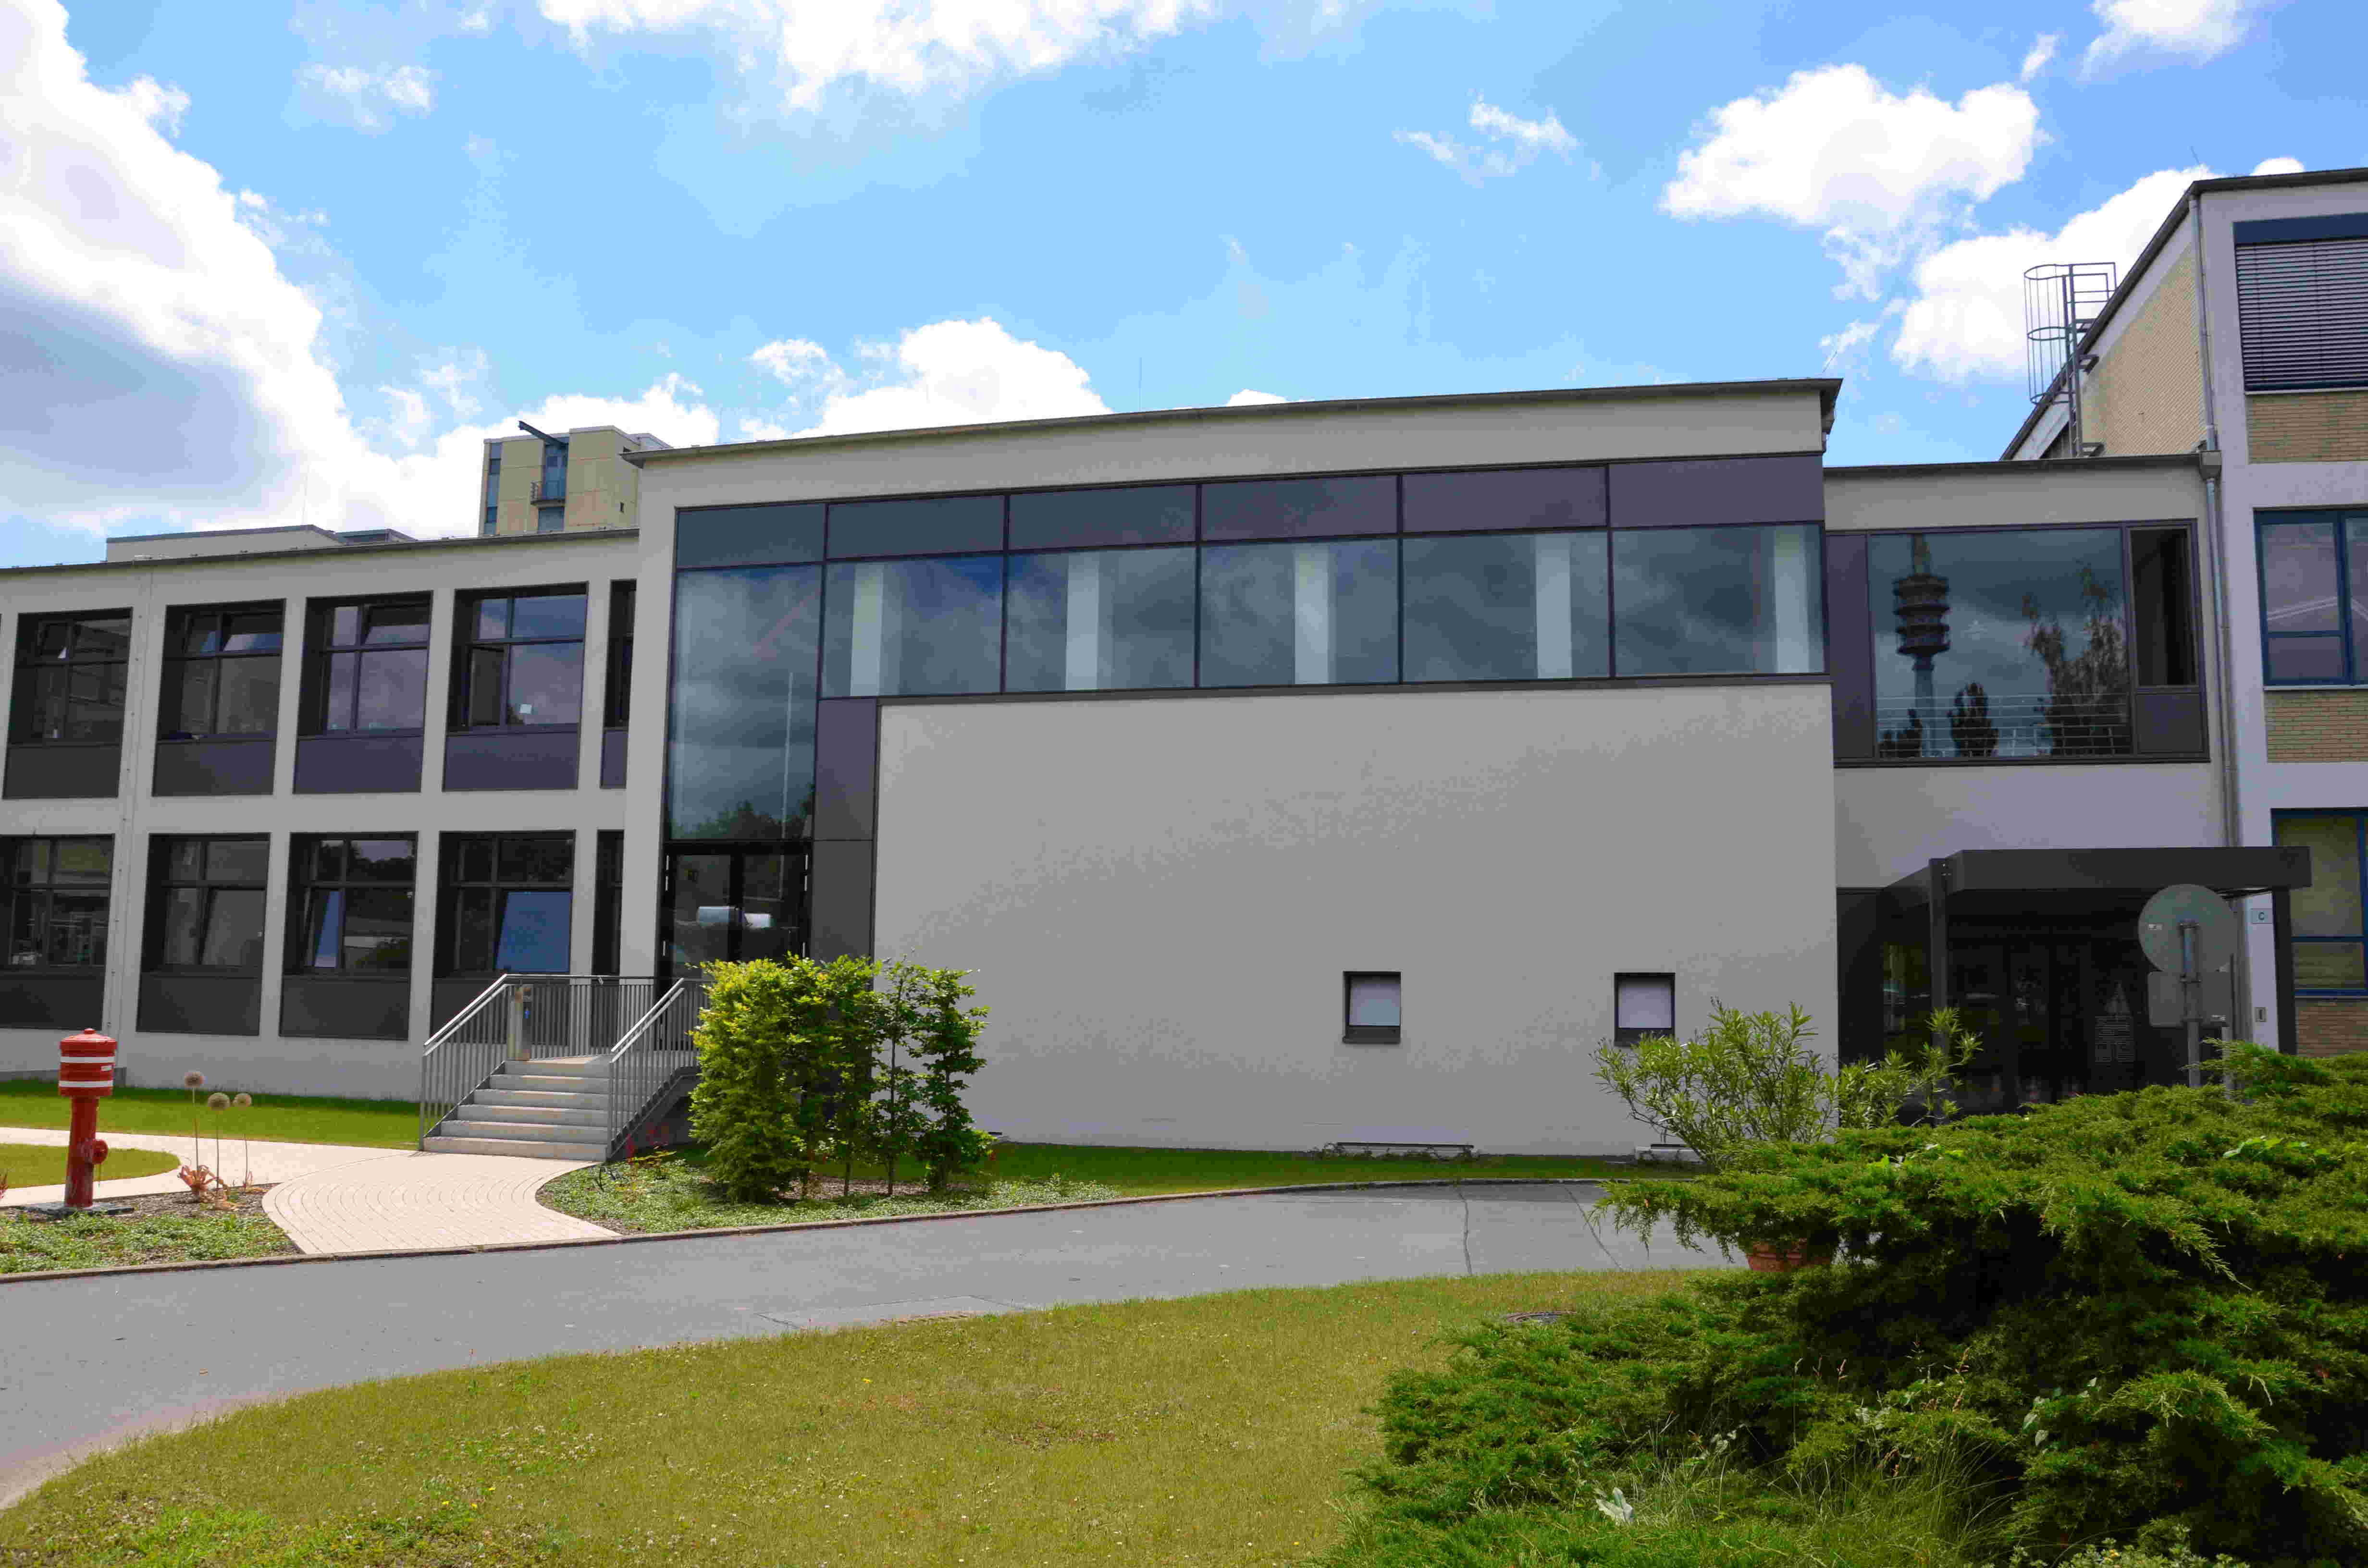
\includegraphics[width = 0.99\textwidth]{Pictures/hzb-2}
\vspace{0.3cm}
\end{column}
\begin{column}{0.59\textwidth}
\centering
``Photon management for femtosecond transient absorption in scattering functional materials'' 
\linebreak
\vskip 0.5cm
\includegraphics[width=0.99\textwidth]{Pictures/test_poster3-2}
\end{column}
\end{columns}
\end{frame}



\section{Robotics Expo \& UMNIK }
\begin{frame}{\quad \quad ~Robotics Expo \& UMNIK}
\centering 
Universal platform for indoor mobile robots -- \newline{}
need for both \textbf{speed} and overcoming \textbf{obstacles}
\newline{}
\begin{columns}
\begin{column}{0.49\textwidth}
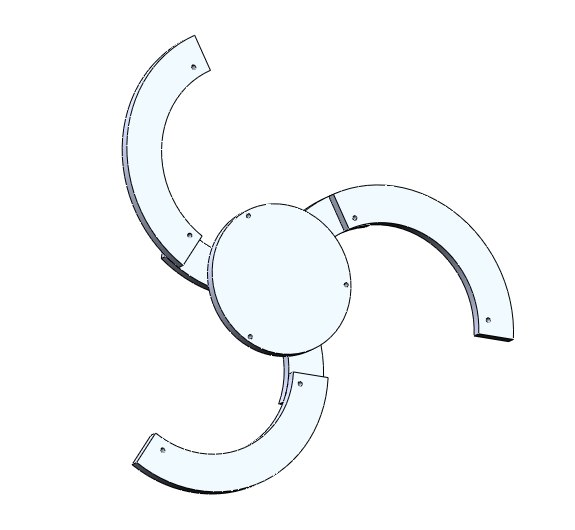
\includegraphics[width=0.9\textwidth]{Pictures/wheel}
\end{column}
\begin{column}{0.49\textwidth}

\includegraphics[height=0.5\textwidth]{Pictures/wheel_closed}
\newline{}
\vskip 0.3cm
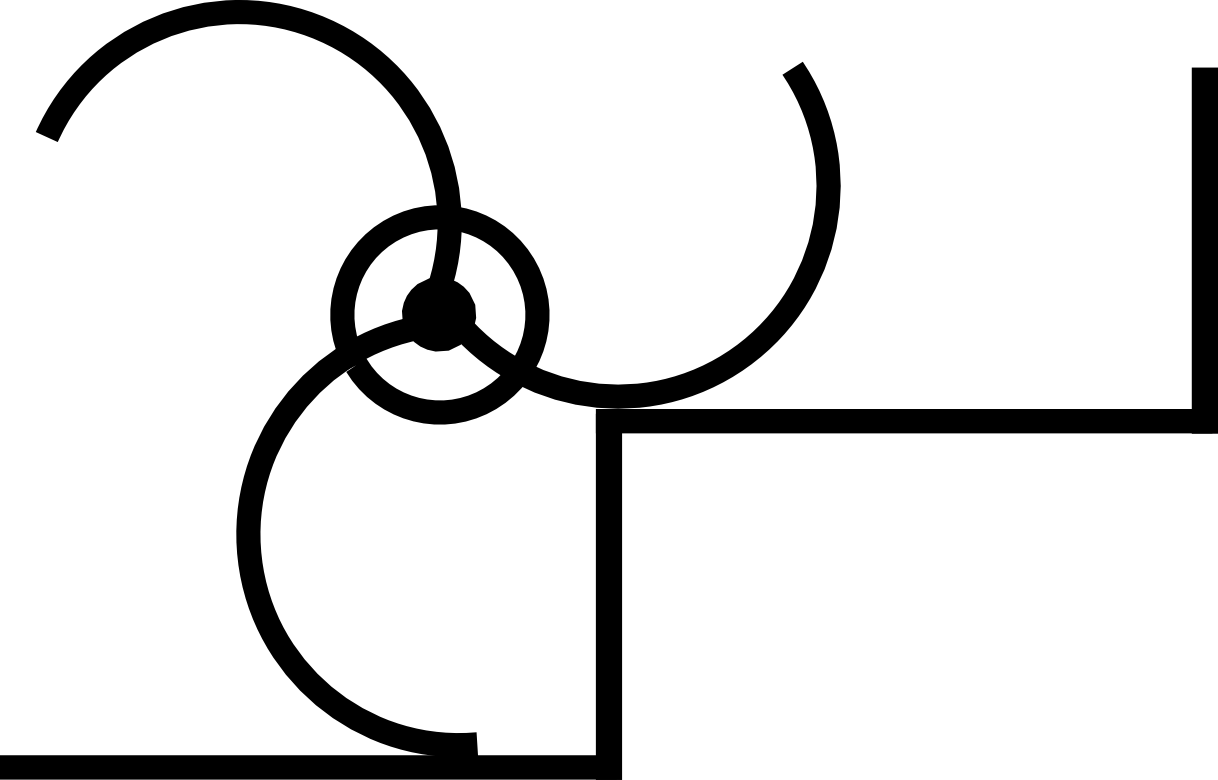
\includegraphics[height=0.5\textwidth]{Pictures/wheel_opened}
\end{column}
\end{columns}
\end{frame}
\section{Eurobot}
\begin{frame}{\quad \quad ~Eurobot}
\centering
\underline{Russian finals participation} -- \textit{no supervisors} 
\newline{}
\vskip 0.3cm
\begin{columns}
\begin{column}{0.39\textwidth}
\begin{itemize}
	\item ROS \& \textsc{Python}
	\item Ubuntu Mate 
	\item Raspberry Pi 3
 	\item Arduino \& \textsc{C++}
 	\item Grip on manipulator
 	\item Balls canon
 	\item Cylinder position detection
 	\item 2 attempts for global navigation \textit{without LIDAR}
\end{itemize}
\end{column}
\begin{column}{0.59\textwidth}
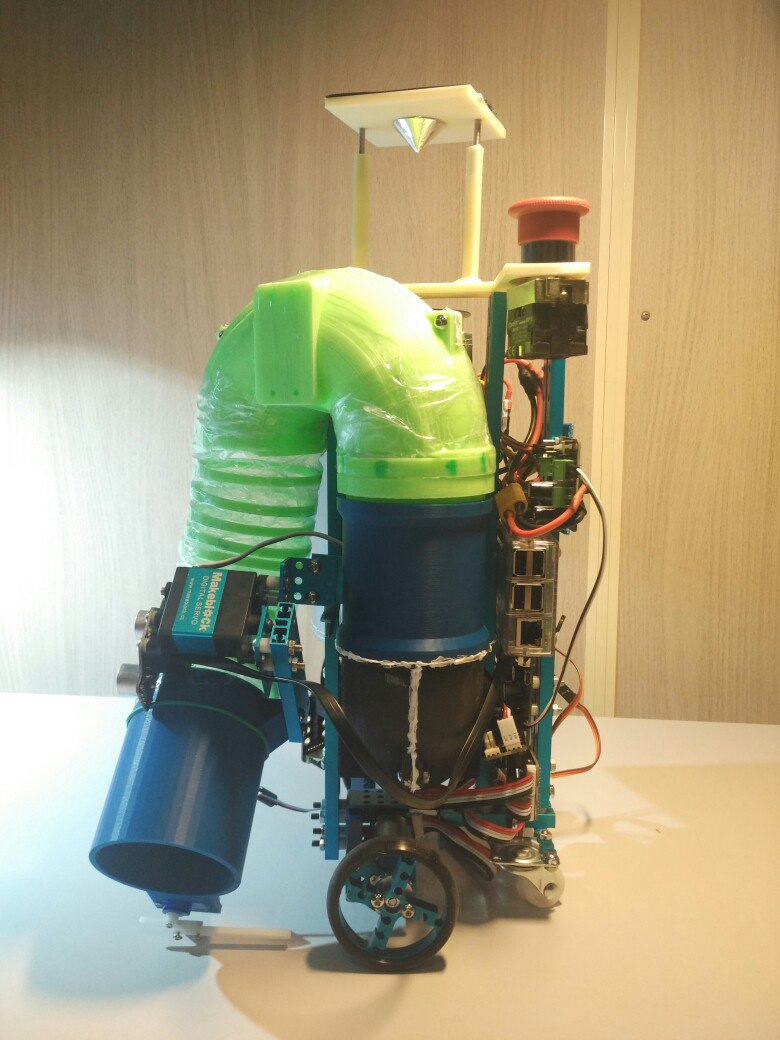
\includegraphics[height=0.6\textwidth]{Pictures/small}
\quad
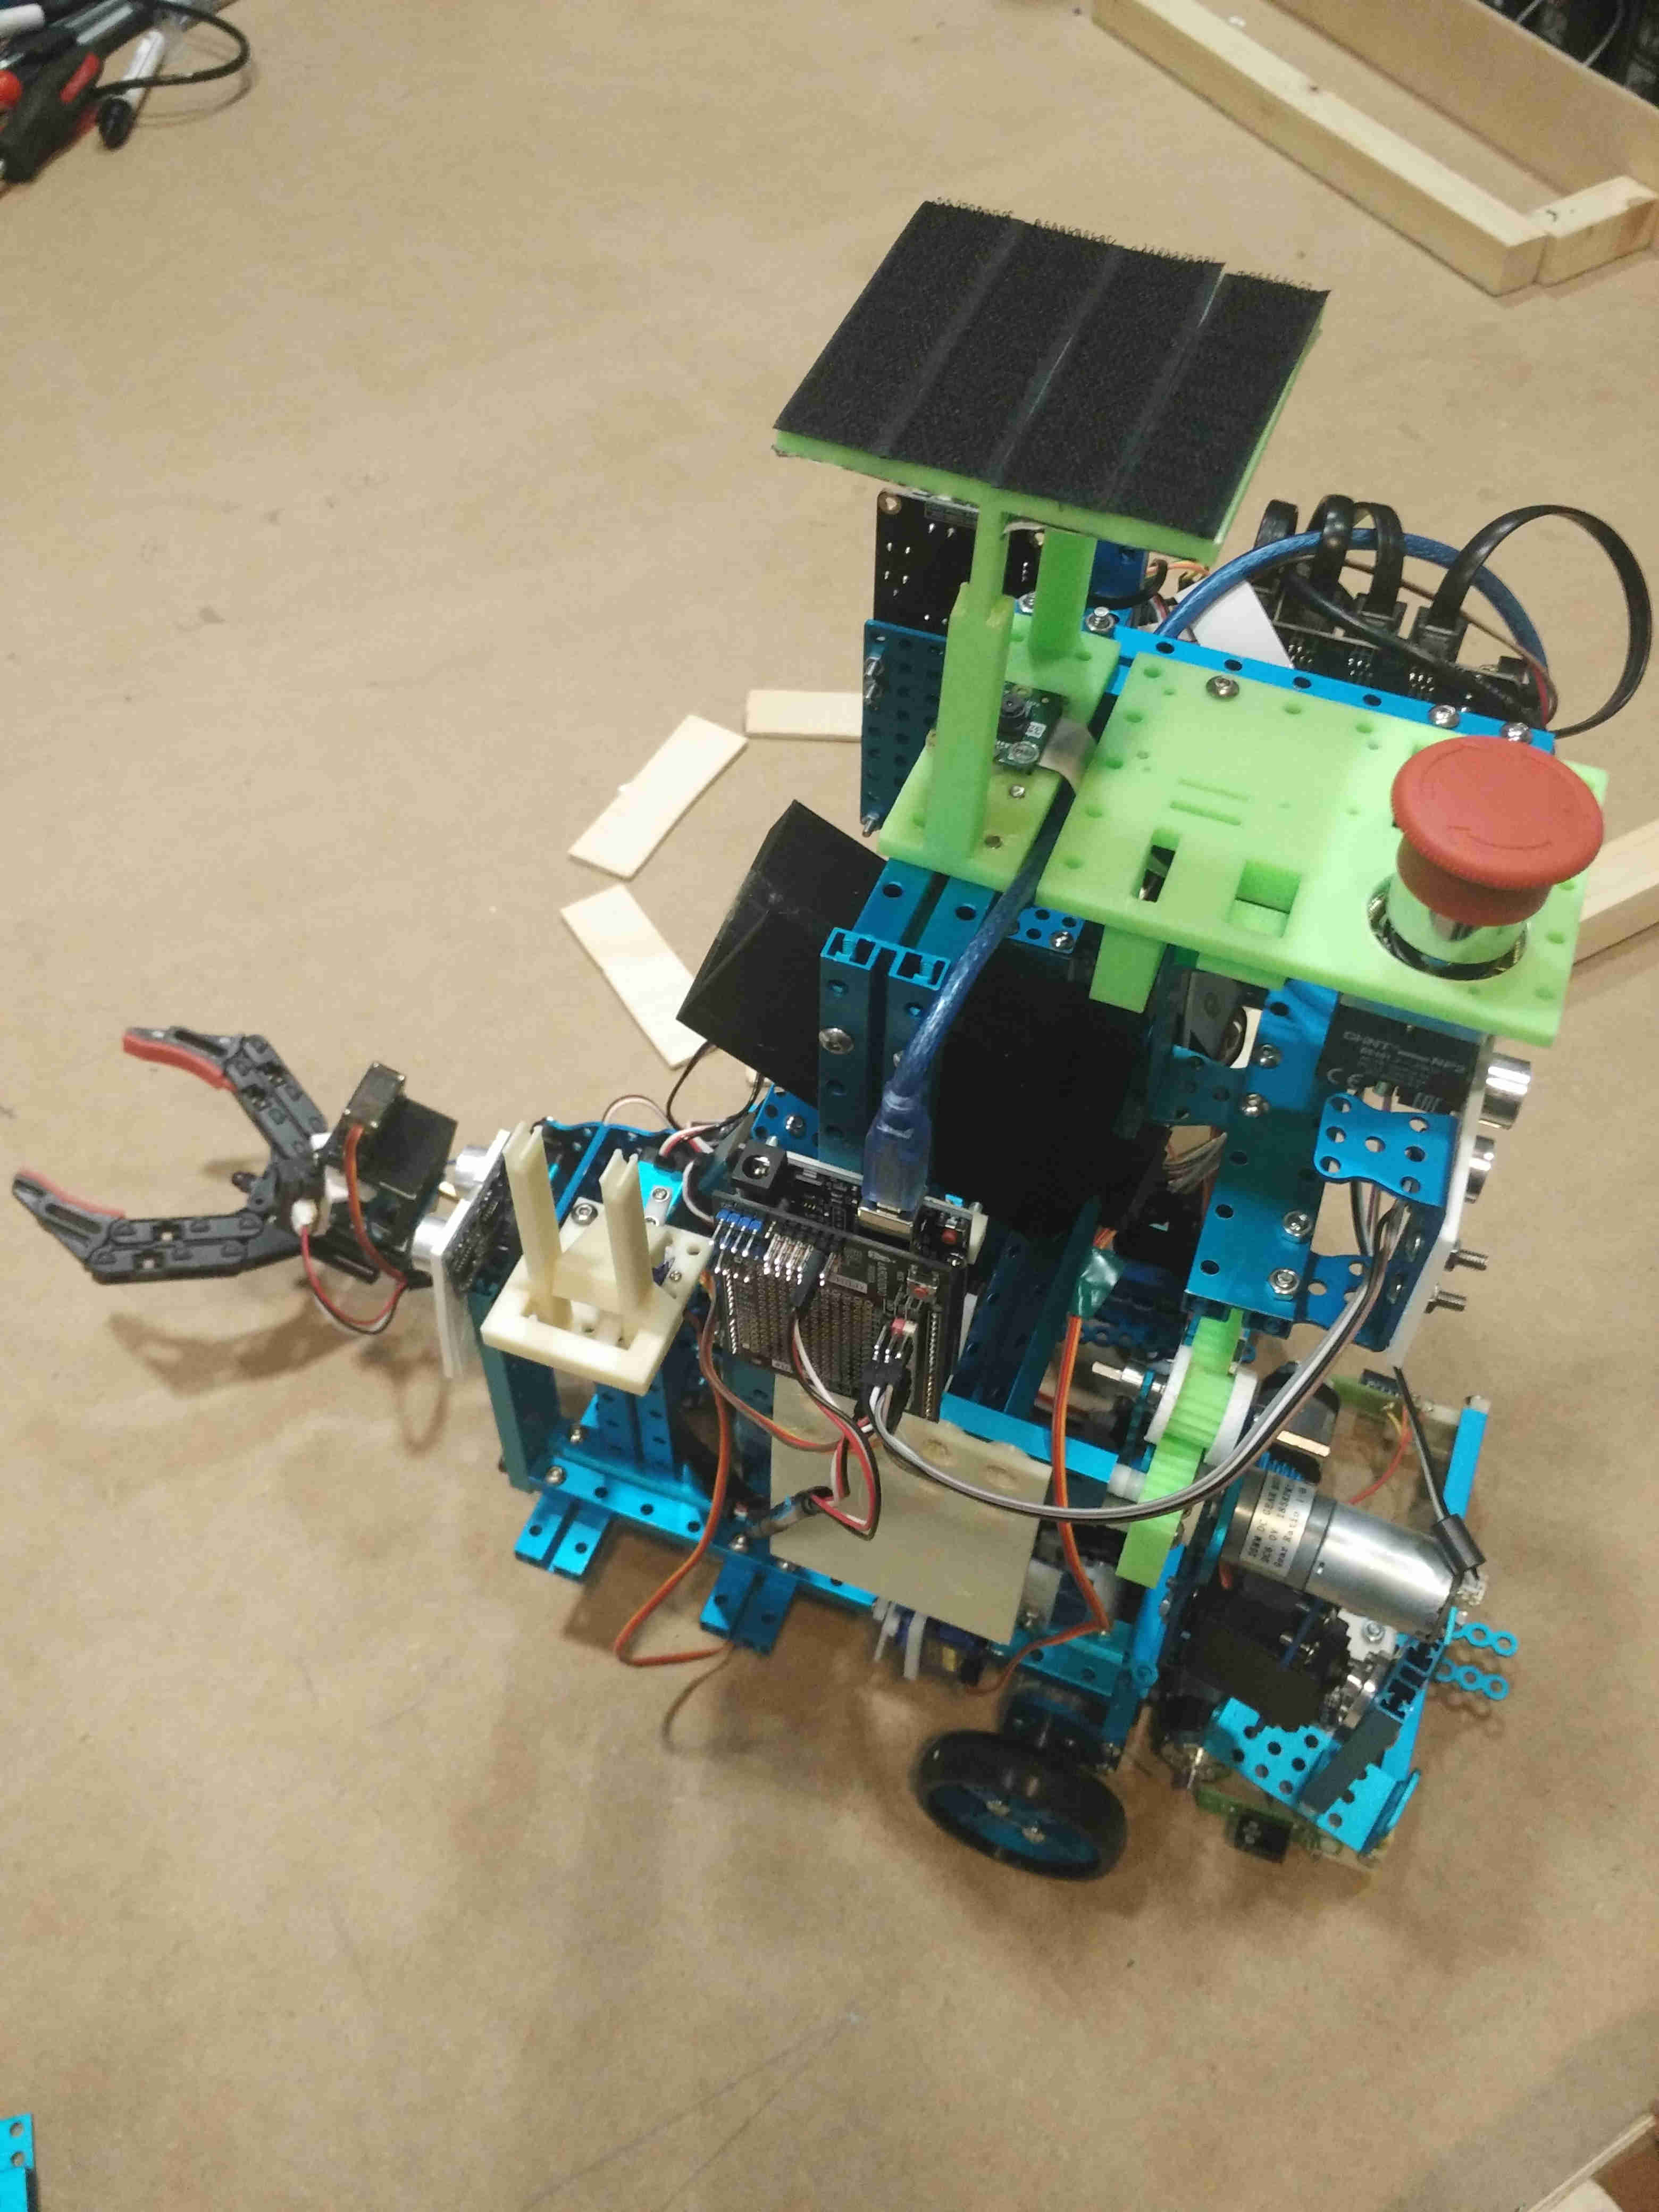
\includegraphics[height=0.6\textwidth]{Pictures/big2}
\end{column}
\end{columns}
\end{frame}

\begin{frame}{\quad \quad ~Global navigations}
\begin{columns}
\begin{column}{0.49\textwidth}
\centering
Ultrasonic time-of-flight measurements
\newline{}
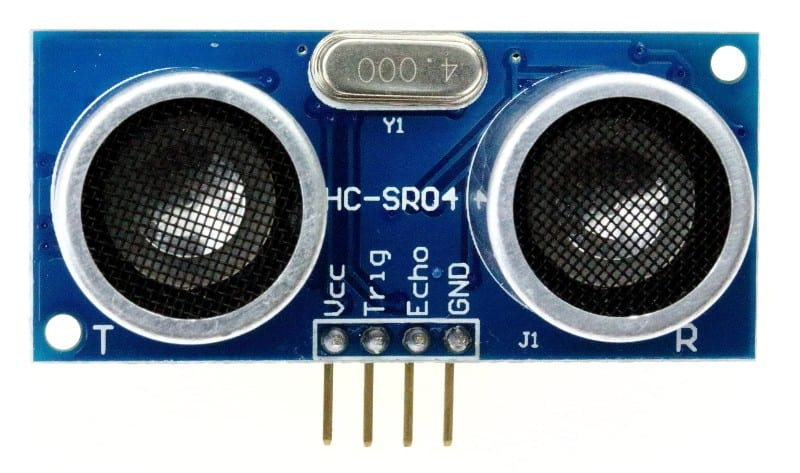
\includegraphics[width = 0.9\textwidth]{Pictures/ultrasonic}
\newline{}

\includegraphics[width = 0.9\textwidth]{Pictures/ultrascheme}
\end{column}
\begin{column}{0.49\textwidth}
\centering
Cone mirror and camera
\newline{}
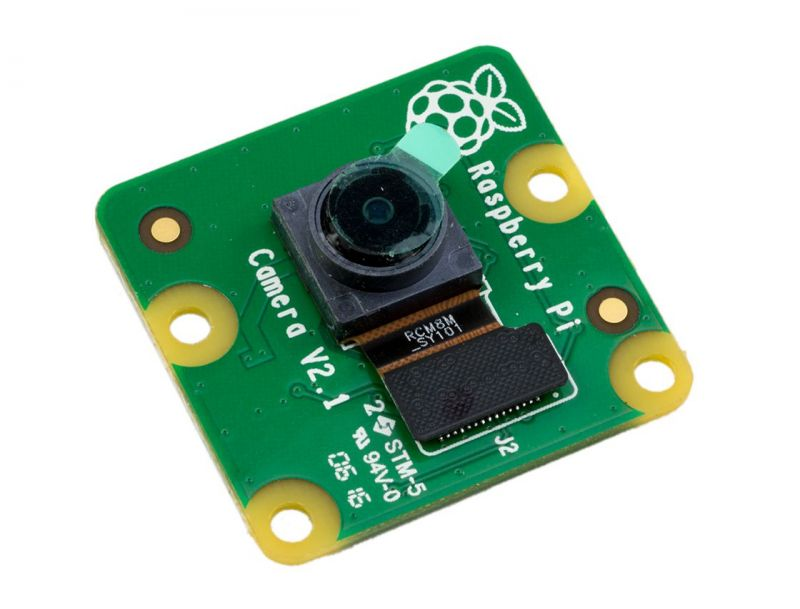
\includegraphics[width = 0.9\textwidth]{Pictures/rpicamera}
\newline{}
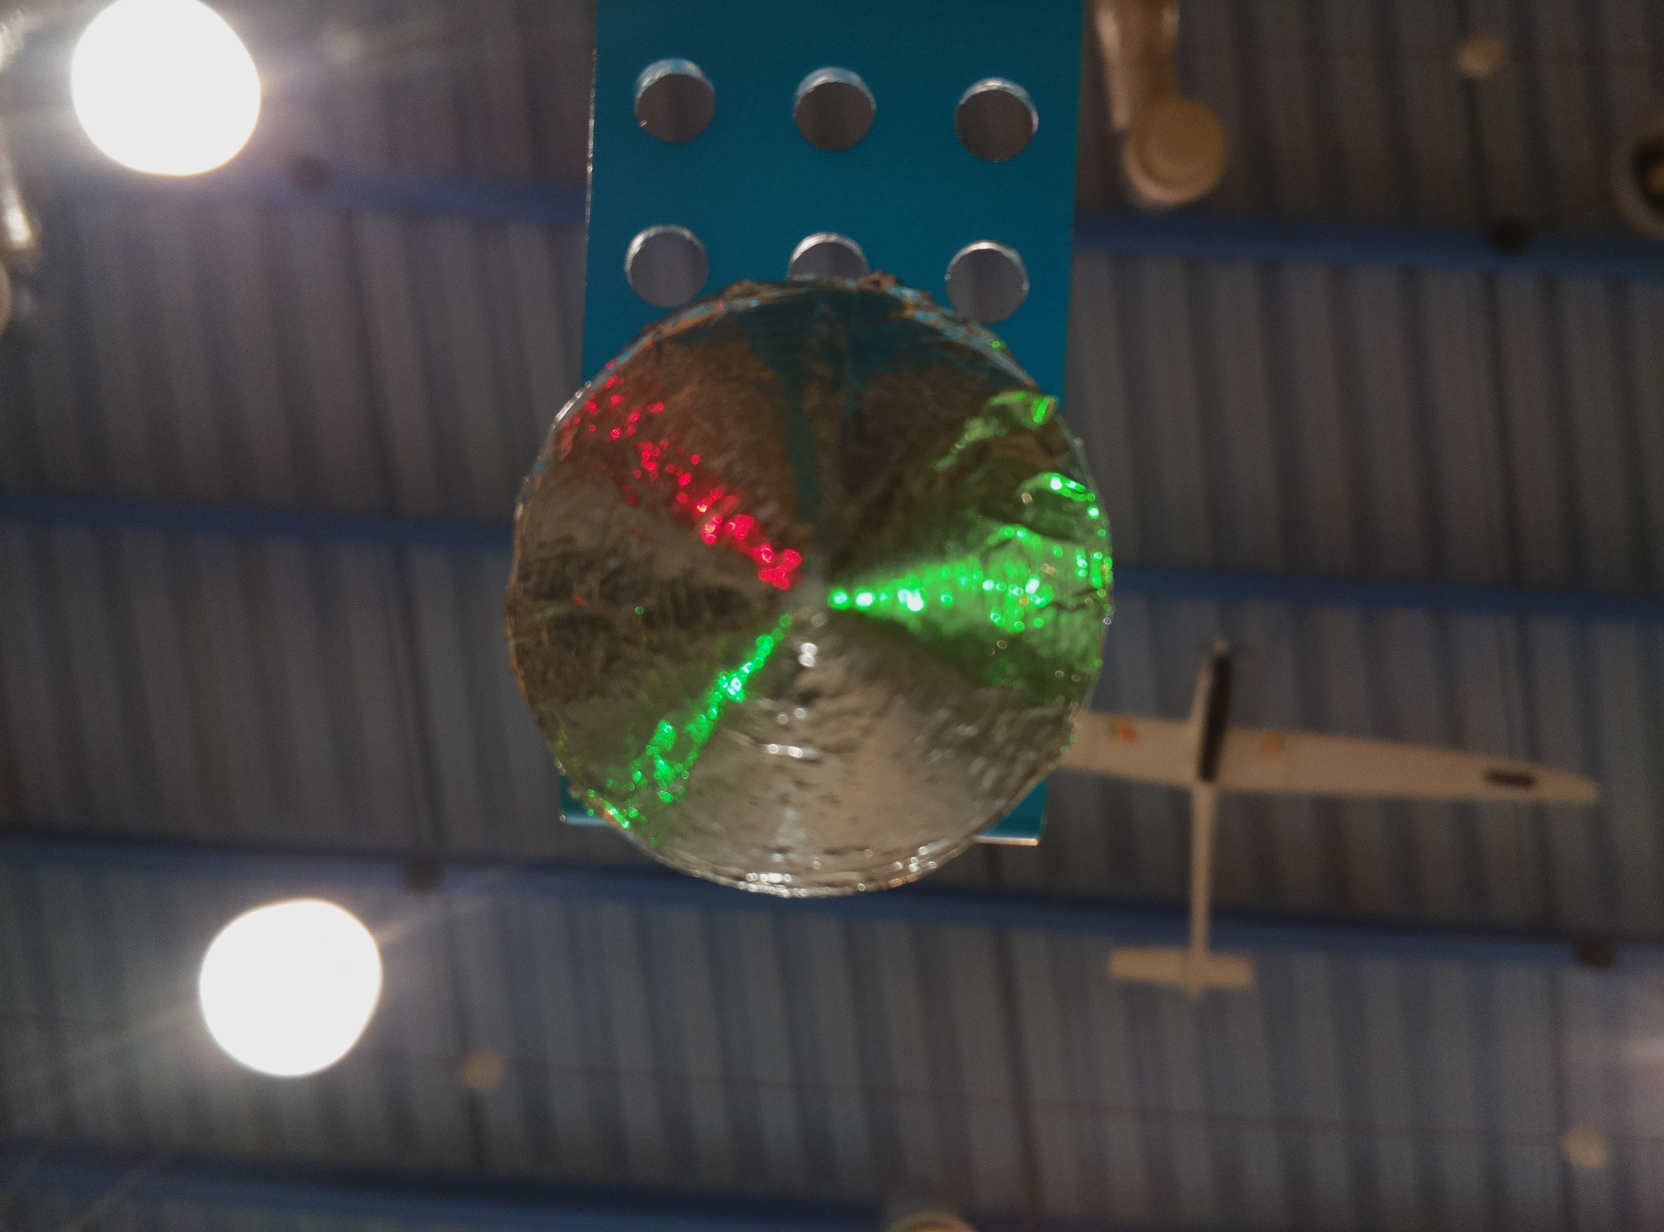
\includegraphics[width = 0.9\textwidth]{Pictures/TestNav}
\end{column}
\end{columns}
\end{frame}

\begin{frame}{\quad \quad ~Eurobot tests}
\begin{columns}
\begin{column}{0.49\textwidth}
\centering
\newline{}
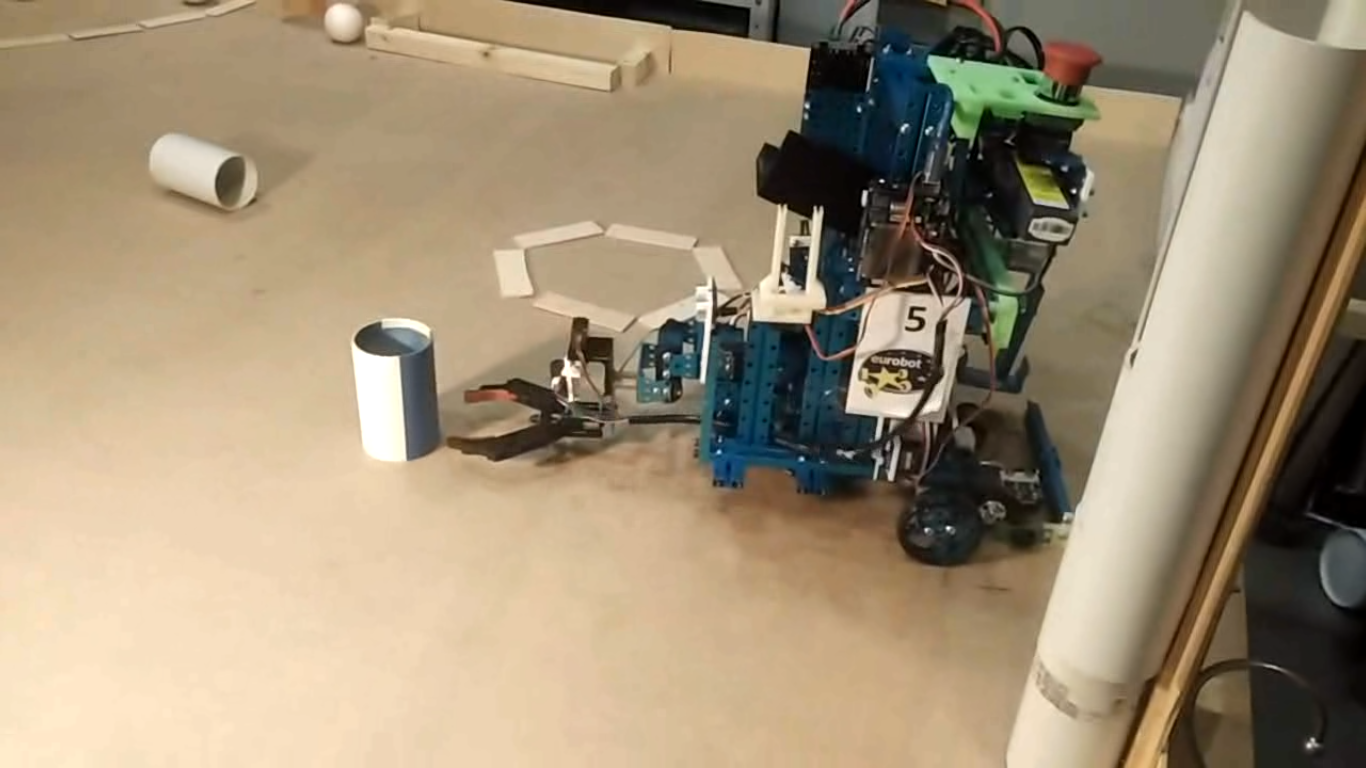
\includegraphics[width = 0.95\textwidth]{Pictures/1}
\vskip 1cm
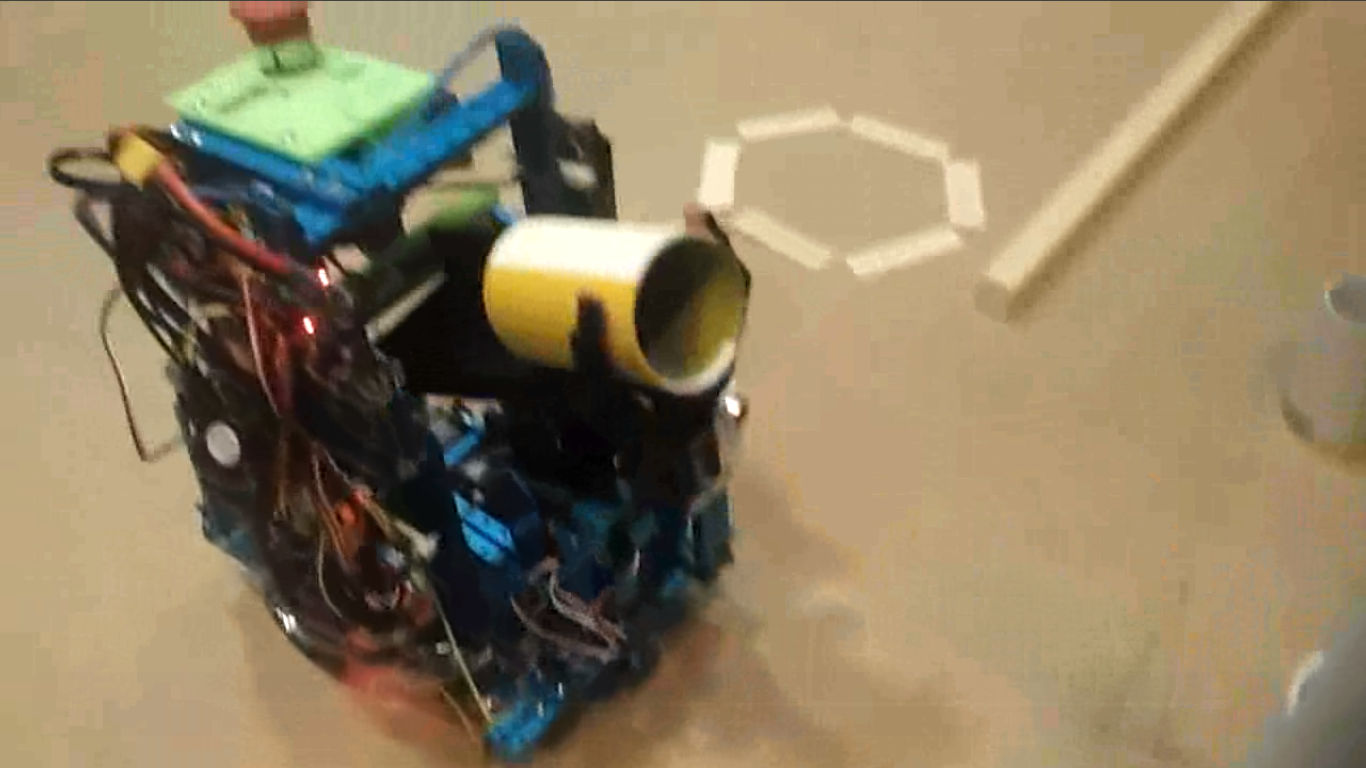
\includegraphics[width = 0.95\textwidth]{Pictures/2}
\end{column}
\begin{column}{0.49\textwidth}
\centering
\newline{}
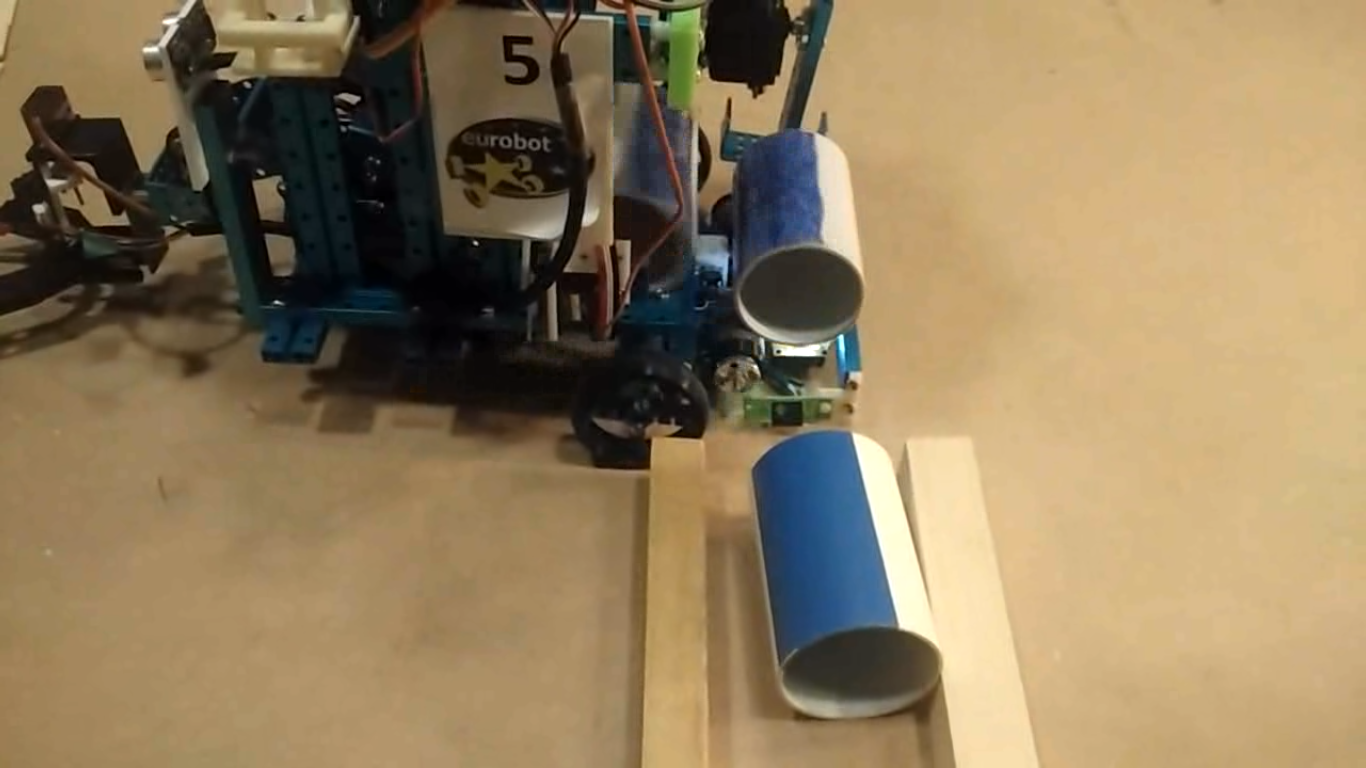
\includegraphics[width = 0.95\textwidth]{Pictures/3}
\vskip 1cm
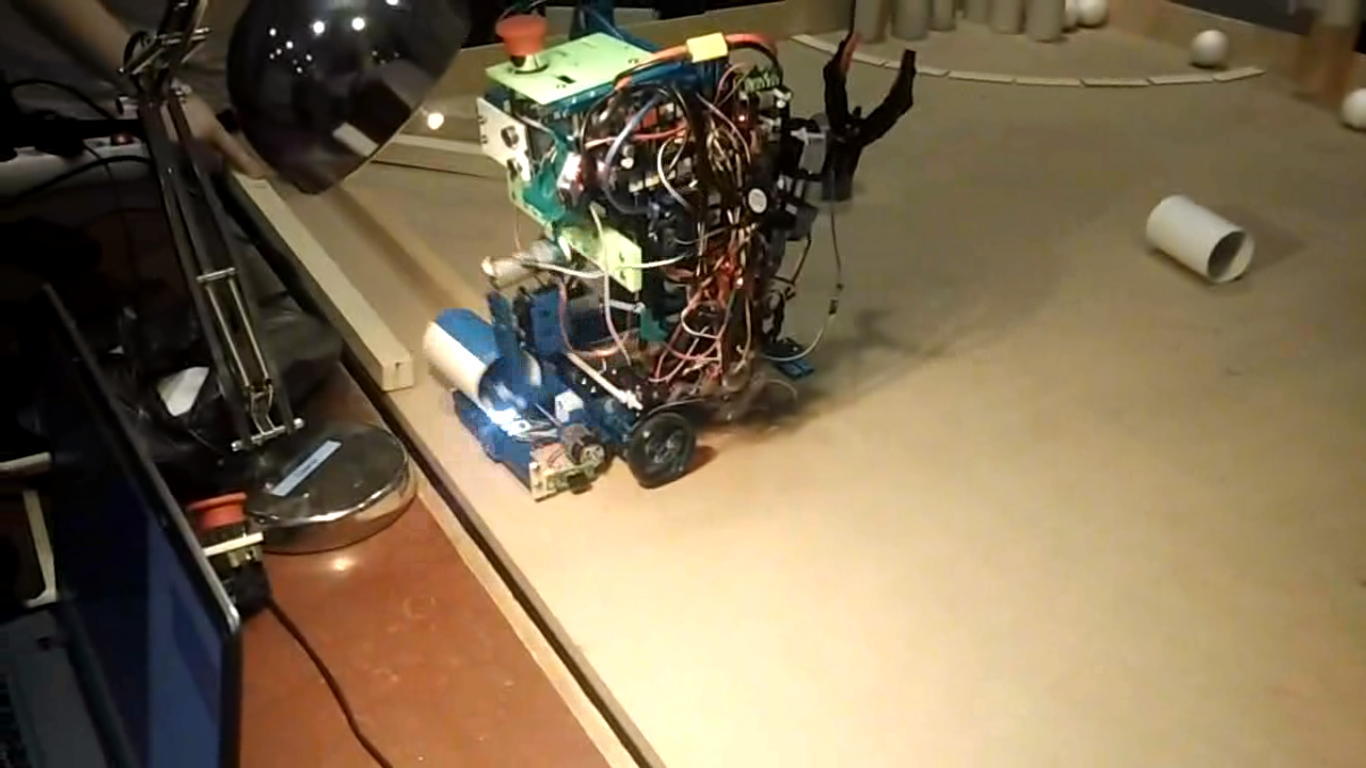
\includegraphics[width = 0.95\textwidth]{Pictures/4}
\end{column}
\end{columns}
\end{frame}
\end{document}
